%_______________________________________________________________________________
\section{Description des paquets scientifiques}
%_______________________________________________________________________________
%_______________________________________________________________________________
\begin{frame}[fragile]
\frametitle{Principales Paquets Scientifiques}
\begin{itemize}
 \item Numpy : essentiel en calcul numérique. 
 \item Matplotlib, Pylab : tracé de figures et fonctions à la matlab.  
 \item Scipy : outils scientifiques spécifiques.  
 \item Maiavi : 3D avancée. 
\end{itemize}
\end{frame}
%_______________________________________________________________________________
%_______________________________________________________________________________
\subsection{Numpy}
%_______________________________________________________________________________
%_______________________________________________________________________________
\begin{frame}[fragile]
\frametitle{Numpy}
\begin{itemize}
 \item \myFig{height=0.5cm}{./fig/numpy-logo.png} : \url{http://www.numpy.org}
 \item \emph{NumPy is the fundamental package for scientific computing with Python}
\end{itemize}
\begin{pythonConsole}
>>> import numpy as np
>>> help(np)

Help on package numpy:

NAME
    numpy

FILE
    /Users/becqg/Library/Enthought/Canopy_64bit/User/lib/python2.7/site-packages
    /numpy/__init__.py

DESCRIPTION
    NumPy
    =====
    
    Provides
      1. An array object of arbitrary homogeneous items
      2. Fast mathematical operations over arrays
      3. Linear Algebra, Fourier Transforms, Random Number Generation
    
...
\end{pythonConsole}
\end{frame}
%_______________________________________________________________________________
%_______________________________________________________________________________
\begin{frame}[fragile]
\frametitle{N-dimensional array Object}
\framesubtitle{}
\begin{itemize}
 \item N-dimensional array : ndarray
 \item Création d'un tableau vide et réservation de l'espace (empty)
 \item Accès aux éléments : A[i, j, \dots]
\end{itemize}
\begin{pythonConsole}

>>> A = numpy.empty((2, 2))
>>> print(A)
[[ -1.28822975e-231   2.68678092e+154]
 [  2.24497156e-314   2.24499315e-314]]
>>> A[0, 0] = 1
>>> A[1, 0] = 2
>>> A[0, 1] = 11
>>> A[1, 1] = 12
>>> print(A)
[[  1.   2.]
 [ 11.  12.]]
>>> type(A)
<type 'numpy.ndarray'>
\end{pythonConsole}
\end{frame}
%_______________________________________________________________________________
%_______________________________________________________________________________
\begin{frame}[fragile]
\frametitle{N-dimensional array Object}
\framesubtitle{}
\begin{itemize}
 \item Rappel : accès aux propiétés et méthodes (dir) 
\end{itemize}
\begin{pythonConsole}

>>> dir(A)
'T', ..., 'all', 'any', 'argmax', 'argmin', 'argpartition', 'argsort', 'astype',
'base', 'byteswap', 'choose', 'clip', 'compress', 'conj', 'conjugate', 'copy',
'ctypes', 'cumprod', 'cumsum', 'data', 'diagonal', 'dot', 'dtype', 'dump',
'dumps', 'fill', 'flags', 'flat', 'flatten', 'getfield', 'imag', 'item',
'itemset', 'itemsize', 'max', 'mean', 'min', 'nbytes', 'ndim', 'newbyteorder',
'nonzero', 'partition', 'prod', 'ptp', 'put', 'ravel', 'real', 'repeat',
'reshape', 'resize', 'round', 'searchsorted', 'setfield', 'setflags', 'shape',
'size', 'sort', 'squeeze', 'std', 'strides', 'sum', 'swapaxes', 'take',
'tofile', 'tolist', 'tostring', 'trace', 'transpose', 'var', 'view'
\end{pythonConsole}
\end{frame}
%_______________________________________________________________________________
%_______________________________________________________________________________
\begin{frame}[fragile]
\frametitle{N-dimensional array Object}
\framesubtitle{Attributs sur la forme du tableau}
\begin{itemize}
 \item Forme du tableau (shape), c'est un tuple.  
 \item Nombre de dimension (ndim)
 \item Type des éléments (dtype)
 \item Taille du tableau (size), c'est le nombre de cellules totales. 
\end{itemize}
\begin{pythonConsole}
>>> A.shape
(2, 2)
>>> (nRow, nCol) = A.shape
>>> nRow = A.shape[0]
>>> nCol = A.shape[1]
>>> A.ndim
2
>>> A.dtype
dtype('float64')
>>> A.size
4
\end{pythonConsole}
\end{frame}
%_______________________________________________________________________________
%_______________________________________________________________________________
\begin{frame}[fragile]
\frametitle{N-dimensional array Object}
\framesubtitle{Changement de forme}
\begin{itemize}
 \item Pour changer la forme (reshape)
 \item Transposition (T)
\end{itemize}
\begin{pythonConsole}
>>> B = A.reshape((4, 1))
array([[  1.],
       [  2.],
       [ 11.],
       [ 12.]])
>>> B.ndim
2
>>> B.size
4
>>> B.T
array([[ 1.,   2.,  11.,  12.]])
\end{pythonConsole}
\end{frame}
%_______________________________________________________________________________
%_______________________________________________________________________________
\begin{frame}[fragile]
\frametitle{N-dimensional array Object}
\framesubtitle{Copie de tableaux}
\begin{itemize}
 \item Les éléments pointés sont liés, seule la forme change.  
 \item Si on veut une copie (copy)
\end{itemize}
\begin{pythonConsole}
>>> B[0, 0] = 21
>>> print(A)
[[ 21.   2.]
 [ 11.  12.]]
>>> B[1, 0]
>>> C = A.copy()
>>> C[0, 0] = 31
>>> print(A[0,0], C[0,0])
(21.0, 31.0)
\end{pythonConsole}
\end{frame}
%_______________________________________________________________________________
%_______________________________________________________________________________
\begin{frame}[fragile]
\frametitle{N-dimensional array Object}
\framesubtitle{Création de tableaux}
\begin{itemize}
 \item tableau vide et réservation de l'espace (empty)
 \item initialisation à zeros (zeros)
 \item initialisation avec des uns (ones)
 \item tableau identité (eye) avec la dimension. 
 \item à partir de listes (array)
 \item suivant une étendue (arange)
\end{itemize}
\begin{pythonConsole}
>>> A = numpy.zeros((2, 4))
>>> print(A)
[[ 0.  0.  0.  0.]
 [ 0.  0.  0.  0.]]
>>> A = numpy.ones((3, 2))
>>> print(A)
[[ 1.  1.]
 [ 1.  1.]
 [ 1.  1.]]
>>> A = numpy.eye(2)
>>> print(A)
[[ 1.  0.]
 [ 0.  1.]]
>>> A = numpy.array([[1, 2], [11, 12]])
>>> print(A)
[[ 1  2]
 [11 12]]
>>> print(numpy.arange(0.5, 1.7, 0.1))
[ 0.5  0.6  0.7  0.8  0.9  1.   1.1  1.2  1.3  1.4  1.5  1.6]
\end{pythonConsole}
\end{frame}
%_______________________________________________________________________________
%_______________________________________________________________________________
\begin{frame}[fragile]
\frametitle{N-dimensional array Object}
\framesubtitle{Types}
\begin{itemize}
 \item Définition du type à la création
 \item Changement de type (astype)
 \item Multiplication ou addition avec un scalaire typé. 
\end{itemize}
\begin{pythonConsole}
>>> A = numpy.array([[1, 2], [11, 12]])
>>> print(A.dtype)
int64
>>> A = numpy.array([[1., 2], [11, 12]])
>>> print(A.dtype)
float64
>>> A = numpy.array([[1, 2], [11, 12]], dtype="float")
>>> print(A.dtype)
float64
>>> A = A.astype("complex")
>>> print(A)
[[  1.+0.j   2.+0.j]
 [ 11.+0.j  12.+0.j]]
>>> A = numpy.array([[1, 2], [11, 12]]) * 1.
>>> print(A.dtype)
float64
\end{pythonConsole}
\end{frame}
%_______________________________________________________________________________
%_______________________________________________________________________________
\begin{frame}[fragile]
\frametitle{N-dimensional array Object}
\framesubtitle{Additions, soustractions, multiplications sur les tableaux}
\begin{itemize}
 \item Addition, soustraction de matrices ou d'un scalaire (+, -)
 \item Multiplication par un scalaire (*)
 \item Produit de matrices élément par élément (*) 
\end{itemize}
\begin{pythonConsole}
>>> A = numpy.array([[1, 2], [11, 12]])
>>> B = numpy.array([[3, 4], [13, 14]])
>>> print(A + 10)
[[ 11.  12.]
 [ 21.  22.]]
>>> print(A + B)
[[  4.   6.]
 [ 24.  26.]]
>>> print(A * 10)
[[  10.   20.]
 [ 110.  120.]]
>>> print(A * B)
[[   3.    8.]
 [ 143.  168.]]
>>> C = numpy.ones((10, ))
>>> print(A * C)
Traceback (most recent call last):
  File £"£<stdin>£"£, line 1, in <module>
ValueError: operands could not be broadcast together with shapes (2,2) (10) 
\end{pythonConsole}
\end{frame}
%_______________________________________________________________________________
%_______________________________________________________________________________
\begin{frame}[fragile]
\frametitle{N-dimensional array Object}
\framesubtitle{Produit scalaire}
\begin{itemize}
 \item Produit scalaire (dot)
 \item See also numpy.dot : en général, pour chaque méthode associée à un ndarray, il existe une fonction équivalente dans numpy. 
\end{itemize}
\begin{pythonConsole}
>>> A = numpy.array([[1, 2], [11, 12]])
>>> B = numpy.array([[3, 4], [13, 14]])
>>> print(A.dot(B))
[[  29.   32.]
 [ 189.  212.]]
>>> print(numpy.dot(A, B))
[[  29.   32.]
 [ 189.  212.]]
>>> C = numpy.ones((10, ))
>>> print(A.dot(C))
Traceback (most recent call last):
  File £"£<stdin>£"£, line 1, in <module>
ValueError: matrices are not aligned
>>> 
\end{pythonConsole}
\end{frame}
%_______________________________________________________________________________
%_______________________________________________________________________________
\begin{frame}[fragile]
\frametitle{N-dimensional array Object}
\framesubtitle{Division}
\begin{itemize}
 \item Division par un scalaire (/)
 \item Division de matrices éléments par éléments (/) 
 \item Attention au type ! 
\end{itemize}
\begin{pythonConsole}
>>> A = numpy.array([[1, 2], [11, 12]])
>>> B = numpy.array([[3, 4], [13, 14]])
>>> print(A/2)
[[0 1]
 [5 6]]
>>> print(A / B)
[[0 0]
 [0 0]]
>>> print(A / B.astype(float))
[[ 0.33333333  0.5       ]
 [ 0.84615385  0.85714286]]
\end{pythonConsole}
\end{frame}
%_______________________________________________________________________________
%_______________________________________________________________________________
\begin{frame}[fragile]
\frametitle{N-dimensional array Object}
\framesubtitle{Autres méthodes}
\begin{itemize}
 \item max, min, sum, mean, std, cumsum, cumprod \dots sur tous les éléments ou sur un axe donné. 
\end{itemize}
\begin{pythonConsole}
>>> A = numpy.ones((2, 3, 4))
>>> print(A.cumsum())
[  1.   2.   3.   4.   5.   6.   7.   8.   9.  10.  11.  12.  13.  14.  15. 
  16.  17.  18.  19.  20.  21.  22.  23.  24.]
>>> print(A.cumsum(axis=0))
[[[ 1.  1.  1.  1.]
  [ 1.  1.  1.  1.]
  [ 1.  1.  1.  1.]]

 [[ 2.  2.  2.  2.]
  [ 2.  2.  2.  2.]
  [ 2.  2.  2.  2.]]]
print(A.cumsum(axis=1))
[[[ 1.  1.  1.  1.]
  [ 2.  2.  2.  2.]
  [ 3.  3.  3.  3.]]

 [[ 1.  1.  1.  1.]
  [ 2.  2.  2.  2.]
  [ 3.  3.  3.  3.]]]
>>> print(A.cumsum(2))
[[[ 1.  2.  3.  4.]
  [ 1.  2.  3.  4.]
  [ 1.  2.  3.  4.]]

 [[ 1.  2.  3.  4.]
  [ 1.  2.  3.  4.]
  [ 1.  2.  3.  4.]]]
\end{pythonConsole}
\end{frame}
%_______________________________________________________________________________
%_______________________________________________________________________________
\begin{frame}[fragile]
\frametitle{N-dimensional array Object}
\framesubtitle{Sélection de sous-tableaux}
\begin{itemize}
 \item découpage slicing, comme pour les séquences.
\end{itemize}
\begin{pythonConsole}
>>> A = numpy.array([[1, 2, 3, 4], [11, 12, 13, 14]])
>>> print(A)
[[ 1  2  3  4]
 [11 12 13 14]]
>>> print(A[1, :])
[11 12 13 14]
>>> print(A[:, 1:3])
[[ 2  3]
 [12 13]]
\end{pythonConsole}
\end{frame}
%_______________________________________________________________________________
%_______________________________________________________________________________
\begin{frame}[fragile]
\frametitle{N-dimensional array Object}
\framesubtitle{Sélection de sous-tableaux}
\begin{itemize}
 \item Comparaison et opérateurs logiques
 \item Opérations logiques pour sélectionner des éléments (masking)
 \item Récupérer les indices (where)
\end{itemize}
\begin{pythonConsole}
>>> A = numpy.array([[1, 2, 3, 4], [11, 12, 13, 14]])
>>> print(A)
[[ 1  2  3  4]
 [11 12 13 14]]
>>> B = A > 2
>>> print(B)
[[False False  True  True]
 [ True  True  True  True]]
>>> print(A[B])
[ 3  4 11 12 13 14]
>>> indices = numpy.where(B)
>>> print(indices[0])
array([0, 0, 1, 1, 1, 1])
>>> print(indices[1])
array([2, 3, 0, 1, 2, 3])
\end{pythonConsole}
\end{frame}
%_______________________________________________________________________________
%_______________________________________________________________________________
\begin{frame}[fragile]
\frametitle{Matrix}
\framesubtitle{}
\begin{itemize}
 \item classe héritée de ndarray avec ndim = 2 et propriétés spéciales.  
\end{itemize}
\begin{pythonConsole}
>>> help(numpy.matrix)
class matrix(numpy.ndarray)
 |  matrix(data, dtype=None, copy=True)
 |  
 |  Returns a matrix from an array-like object, or from a string of data.
 |  A matrix is a specialized 2-D array that retains its 2-D nature
 |  through operations.  It has certain special operators, such as £`££`£*£`££`£
 |  (matrix multiplication) and £`££`£**£`££`£ (matrix power).
...

>>> A = numpy.matrix([[1, 2], [11, 12]])
>>> print(A)
[[ 1  2]
 [11 12]]
>>> type(A)
 <class 'numpy.matrixlib.defmatrix.matrix'>
>>> A = numpy.matrix("[1, 2, 3, 4; 11, 12, 13, 14]")
>>> print(A)
[[ 1  2  3  4]
 [11 12 13 14]]
\end{pythonConsole}
\end{frame}
%_______________________________________________________________________________
%_______________________________________________________________________________
\begin{frame}[fragile]
\frametitle{Matrix}
\framesubtitle{}
\begin{itemize}
 \item Saisie type ndarray avec des listes imbriquées. 
 \item Possibilité de saisie type Matlab.
\end{itemize}
\begin{pythonConsole}
>>> help(numpy.matrix)
>>> A = numpy.matrix([[1, 2], [11, 12]])
>>> print(A)
[[ 1  2]
 [11 12]]
>>> type(A)
 <class 'numpy.matrixlib.defmatrix.matrix'>
>>> A = numpy.matrix("[1, 2, 3, 4; 11, 12, 13, 14]")
>>> print(A)
[[ 1  2  3  4]
 [11 12 13 14]]
\end{pythonConsole}
\end{frame}
%_______________________________________________________________________________
%_______________________________________________________________________________
\begin{frame}[fragile]
\frametitle{Matrix}
\framesubtitle{Multiplication et exposant}
\begin{itemize}
 \item Produit de matrices (*)
 \item Exposant de matrice (**)
\end{itemize}
\begin{pythonConsole}
>>> A = numpy.matrix([[1, 2], [11, 12]])
>>> B = numpy.matrix([[3, 4], [13, 14]])
>>> print(A * B)
[[ 29  32]
 [189 212]]
>>> print(A ** 2)
[[ 23  26]
 [143 166]]
\end{pythonConsole}
\end{frame}
%_______________________________________________________________________________
%_______________________________________________________________________________
\begin{frame}[fragile]
\frametitle{Matrix}
\framesubtitle{Opérateurs matriciels courants}
\begin{itemize}
 \item Transposition (T)
 \item Inversion (I)
 \item Opérateur Hermitien (H)
\end{itemize}
\begin{pythonConsole}
>>> A = numpy.matrix([[1, 2], [11, 12]])
>>> print(A)
[[ 1  2]
 [11 12]]
>>> print(A.T)
[[ 1 11]
 [ 2 12]]
>>> print(A.I)
print(A.I)
[[-1.2  0.2]
 [ 1.1 -0.1]]
>>> B = numpy.matrix([[1, 2+1j], [11+1j, 12]])
>>> print(B)
[[  1.+0.j   2.+1.j]
 [ 11.+1.j  12.+0.j]]
>>> print(B.H)
[[  1.-0.j  11.-1.j]
 [  2.-1.j  12.-0.j]]
\end{pythonConsole}
\end{frame}
%_______________________________________________________________________________
%_______________________________________________________________________________
% 
% frame
%

\begin{frame}[fragile]
\frametitle{Numpy}
\framesubtitle{Tableaux ND et fonctions associ\'ees}

\begin{itemize}
 \item Les exemples sont donnés dans IPython avec les fonctions Pylab chargées.  
\end{itemize}

\begin{pythonConsole}
>>> A = array([[1,2,3],[4,5,6],[7,8,9]])
>>> whos

Variable   Type       Data/Info
-------------------------------
A          ndarray    3x3: 9 elems, type `int64`, 72 bytes

>>> A
array([[1, 2, 3],
       [4, 5, 6],
       [7, 8, 9]])
       
>>> A.size
9

>>> A.shape
(3,3)

>>> B = array([[1,0,0],[0,1,0],[0,0,1]])

>>> A*B

array([[ 1.,  0.,  0.],
       [ 0.,  5.,  0.],
       [ 0.,  0.,  9.]])
\end{pythonConsole}
\end{frame}

% 
% frame
% 

\begin{frame}
\frametitle{Numpy}
\framesubtitle{Tableaux ND et fonctions associ\'ees}
$\bullet$ M\'ethodes
\begin{itemize}
\item nonzero, max, min, mean, std ...
\item sum, cumprod, cumsum ...
\item reshape, resize, flatten, transpose ... 
\end{itemize}
\vspace{0.5cm}
$\bullet$ Fonctions
\begin{itemize}
\item $*$ : produit \'elt./\'elt.
\item $dot(.,.)$ : produit matriciel
\item ...
\end{itemize}
\end{frame}
%
% frame
%
\begin{frame}[fragile]
\frametitle{Numpy}
\framesubtitle{NDarray {\em vs.} matrix}
\begin{pythonConsole}
>>> A = array([[1.,2,3],[4,5,6],[7,8,9]])
>>> B = array([[1,0,0],[0,1,0],[0,0,1]])
>>> C = matrix([[1.,2,3],[4,5,6],[7,8,9]])
>>> D = matrix([[1,0,0],[0,1,0],[0,0,1]])

>>> whos
Variable   Type       Data/Info
-------------------------------
A          ndarray    3x3: 9 elems, type `float64`, 72 bytes
B          ndarray    3x3: 9 elems, type `int64`, 72 bytes
C          matrix     [[ 1.  2.  3.]\n [ 4.  5.  6.]\n [ 7.  8.  9.]]
D          matrix     [[1 0 0]\n [0 1 0]\n [0 0 1]]

>>> dot(A,B)

array([[ 1.,  2.,  3.],
       [ 4.,  5.,  6.],
       [ 7.,  8.,  9.]])

>>>  C*D

matrix([[ 1.,  2.,  3.],
        [ 4.,  5.,  6.],
        [ 7.,  8.,  9.]])

\end{pythonConsole}
\end{frame}

% 
% Slide
% 

\begin{frame}[fragile]
\frametitle{Numpy}
\framesubtitle{matrix}
$\bullet$ M\'ethodes
\begin{itemize}
\item min, max, mean, std, ...
\item .T, .H, .I, ...
\item reshape, flatten, ...
\end{itemize}
\vspace{0.2cm}
$\bullet$ Fonctions
\begin{itemize}
\item inv, svd, eig, ...
\end{itemize}
\vspace{0.2cm}
\underline{Diff\'erences entre array et matrix}
\begin{pythonConsole}
>>> A = array([[1.,2,3],[4,5,6],[7,8,9]])
>>> B = matrix([[1.,2,3],[4,5,6],[7,8,9]])

>>> A**2
array([[  1.,   4.,   9.],
       [ 16.,  25.,  36.],
       [ 49.,  64.,  81.]])

>>> B**2
matrix([[  30.,   36.,   42.],
        [  66.,   81.,   96.],
        [ 102.,  126.,  150.]])

\end{pythonConsole}
\end{frame}
%...............................................................................
%
% frame
%
%...............................................................................
\begin{frame}[fragile]
\frametitle{Numpy}
\framesubtitle{NDarray {\em vs.} matrix}
\begin{pythonConsole}
>>> A = array([[1.,2,3],[4,5,6],[7,8,9]])
>>> B = array([[1,0,0],[0,1,0],[0,0,1]])
>>> C = matrix([[1.,2,3],[4,5,6],[7,8,9]])
>>> D = matrix([[1,0,0],[0,1,0],[0,0,1]])

>>> whos
Variable   Type       Data/Info
-------------------------------
A          ndarray    3x3: 9 elems, type `float64`, 72 bytes
B          ndarray    3x3: 9 elems, type `int64`, 72 bytes
C          matrix     [[ 1.  2.  3.]\n [ 4.  5.  6.]\n [ 7.  8.  9.]]
D          matrix     [[1 0 0]\n [0 1 0]\n [0 0 1]]

>>> dot(A,B)

array([[ 1.,  2.,  3.],
       [ 4.,  5.,  6.],
       [ 7.,  8.,  9.]])

>>>  C*D

matrix([[ 1.,  2.,  3.],
        [ 4.,  5.,  6.],
        [ 7.,  8.,  9.]])

\end{pythonConsole}
\end{frame}
%...............................................................................
%
% frame
%
%...............................................................................
\begin{frame}[fragile]
\frametitle{Numpy}
\framesubtitle{matrix}
$\bullet$ M\'ethodes
\begin{itemize}
\item min, max, mean, std, ...
\item .T, .H, .I, ...
\item reshape, flatten, ...
\end{itemize}
\vspace{0.2cm}
$\bullet$ Fonctions
\begin{itemize}
\item inv, svd, eig, ...
\end{itemize}
\vspace{0.2cm}
\underline{Diff\'erences entre array et matrix}
\begin{pythonConsole}
>>> A = array([[1.,2,3],[4,5,6],[7,8,9]])
>>> B = matrix([[1.,2,3],[4,5,6],[7,8,9]])

>>> A**2
array([[  1.,   4.,   9.],
       [ 16.,  25.,  36.],
       [ 49.,  64.,  81.]])

>>> B**2
matrix([[  30.,   36.,   42.],
        [  66.,   81.,   96.],
        [ 102.,  126.,  150.]])

\end{pythonConsole}
\end{frame}
%...............................................................................
%_______________________________________________________________________________
%_______________________________________________________________________________
\subsection{Matplotlib}
%...............................................................................
\begin{frame}[fragile]
\frametitle{Matplotlib}
\framesubtitle{Librairie graphique}
\begin{itemize}
\item Outils graphiques 2D
\item Toolkits : Basemap, Axesgrid, mplot3d
\item Beaucoup d'exemples : www.matplotlib.org
\end{itemize}
\begin{minipage}{0.68\linewidth}
\begin{pythonConsole}
>>> t=arange(0,1,10e-5)
>>> S1=sin(2*pi*2*t);S2=sin(2*pi*7*t+(3*pi/7)),
>>> fig=figure()
>>> ax=fig.add_subplot(111,xlim=(-1,1),ylim=(-1,1))
>>> courbe=ax.plot(S1,S2);ax.grid('on')
>>> annotate('Courbe',xy=(-0.5,0.5),xytext=(-0.65,0),\
       bbox=dict(boxstyle='round,pad=0.5',fc='red',\ 
       alpha=0.2),arrowprops=dict(arrowstyle='->',\
         connectionstyle='arc3,rad=0'))
>>> title(r"Figure de Lissajous ($\nu_1=2$, $\nu_2=1$,\
         $\phi=\frac{3\pi}{7}$)")
>>> xlabel(r"$\sin(2\pi\nu_1 t)$")
>>> ylabel(r"$\sin(2\pi\nu_2 t + \phi)$")
>>> show()

\end{pythonConsole}
\end{minipage}
\begin{minipage}{0.3\linewidth}
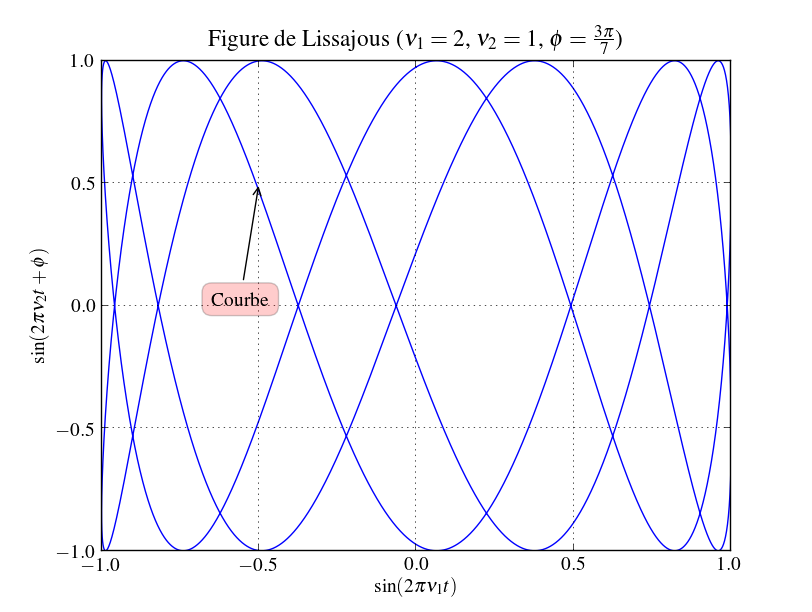
\includegraphics[width=4.5cm,height=4.5cm]{fig/Lissajous.png}
\end{minipage}
\end{frame}

% 
% Slide
% 

\begin{frame}[fragile]
\frametitle{Matplotlib}
\framesubtitle{Exemples}
\begin{minipage}{0.58\linewidth}
\begin{pythonConsole}
>>> [X,Y] = meshgrid(linspace(-2,2,500),\
linspace(-2,2,500))
>>> Z=X+Y*1j
>>> k=1
>>> while k<=75:
>>> 	Z = Z - (Z/3 - 1) / (3*Z**2)
>>>	k=k+1
>>> close('all')	
>>> imshow(angle(Z),cmap=cm.gray)
>>> #savefig('/MonChemin/Lenom.pdf',format='pdf')
>>> show()
\end{pythonConsole}
\end{minipage}
%\hspace{0.5cm}
\begin{minipage}{0.4\linewidth}
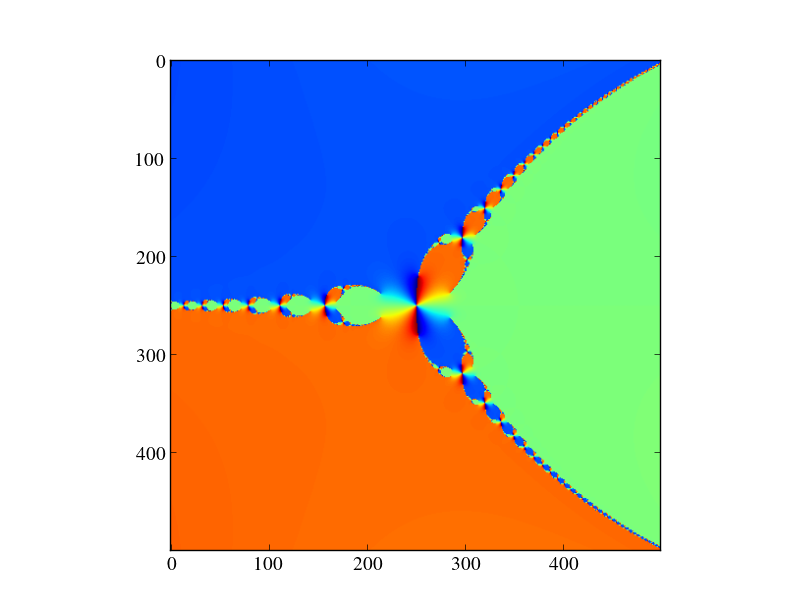
\includegraphics[width=5.5cm,height=4.5cm]{fig/fractal.png}
\end{minipage}
\end{frame}

% 
% Slide
% 
\begin{frame}
\frametitle{Matplotlib}
\framesubtitle{Exemples}

\begin{minipage}{0.4\linewidth}
\begin{figure}
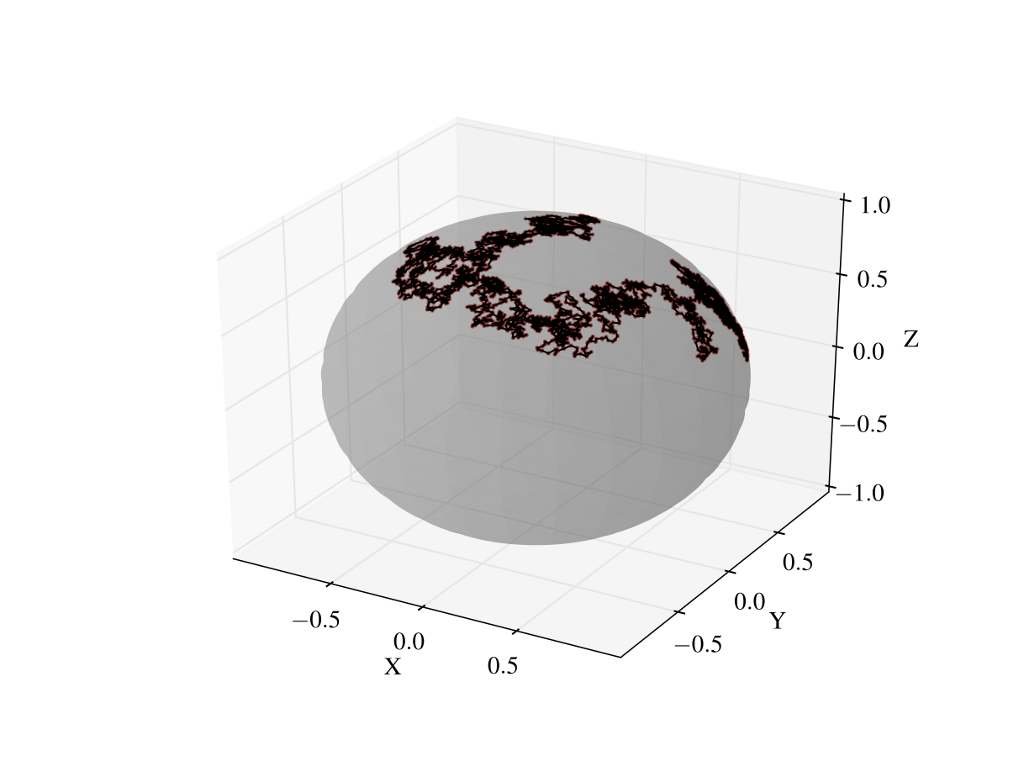
\includegraphics[width=6.5cm,height=5.5cm]{fig/BrownSphere.png}
\end{figure}
\end{minipage}
\hspace{1cm}
\begin{minipage}{0.4\linewidth}
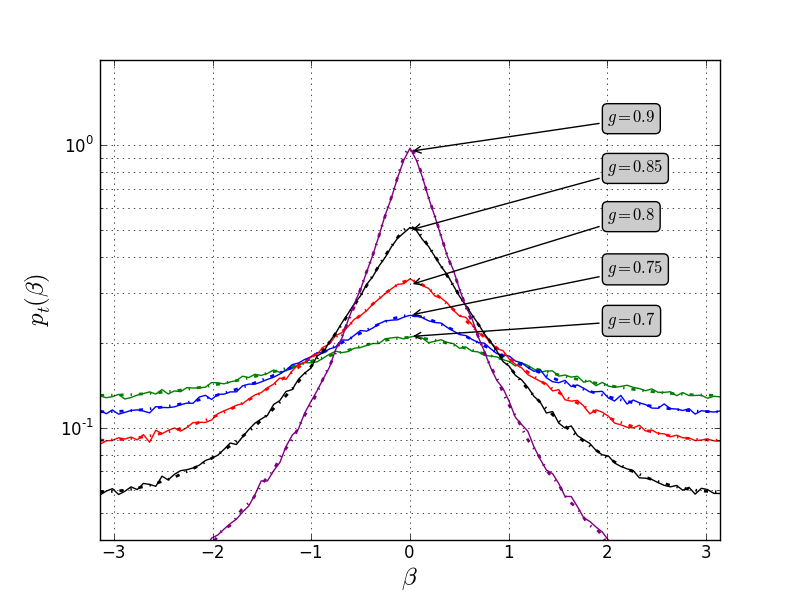
\includegraphics[width=5.5cm,height=4.5cm]{fig/Distrib.png}
\end{minipage}
\end{frame}
%...............................................................................
%_______________________________________________________________________________
%_______________________________________________________________________________
\subsection{Pylab}
%...............................................................................
\begin{frame}[fragile]
\frametitle{Pylab}
\framesubtitle{}
\begin{itemize}
 \item Module de Matplotlib : matplotlib\slash{}pylab.py
 \item Redéfinit des fonctions à la Matlab.
 \item Raccourci : "import pylab" au lieu de "import matplotlib.pylab"
 \item En général, et exceptionnellement, s'utilise : "from pylab import *" 
\end{itemize}
\begin{pythonConsole}
>>> from pylab import *
>>> plot([1, 5, 2, 4, 3])
[<matplotlib.lines.Line2D object at 0x4ec05b0>]
>>> show()
>>> a = randn(100, 10)
>>> type(a)
<type 'numpy.ndarray'>
>>> a.shape
(100, 10)
>>> help(matplotlib.pylab)
\end{pythonConsole}
\end{frame}
%...............................................................................
%_______________________________________________________________________________
%_______________________________________________________________________________
\subsection{Scipy}
%...............................................................................
\begin{frame}
\frametitle{Scipy}
\framesubtitle{Scientific library}
\begin{itemize}
 \item \myFig{height=0.5cm}{./fig/scipy-logo.png}\ : http://www.scipy.org 
\end{itemize}
\begin{center}
\tiny
\begin{tabular}{p{3cm}p{2cm}|p{3cm}p{2cm}}
Clustering package & scipy.cluster & Constants & scipy.constants \\
Discrete Fourier transforms & scipy.fftpack & Integration and ODEs & scipy.integrate \\
Interpolation & scipy.interpolate & Input and output & scipy.io \\
Linear algebra & scipy.linalg & Miscellaneous routines & scipy.misc \\
Multi-dimensional image processing & scipy.ndimage & Orthogonal distance regression & scipy.odr \\
Optimization and root finding & scipy.optimize & {\bfseries Signal processing} & scipy.signal \\
Sparse matrices & scipy.sparse & Sparse linear algebra & scipy.sparse.linalg \\
Compressed Sparse Graph Routines & scipy.sparse.csgraph & Spatial algorithms and data structures & scipy.spatial \\
Special functions & scipy.special & Statistical functions & scipy.stats \\
Statistical functions for masked arrays & scipy.stats.mstats & 
C/C++ integration & scipy.weave \\
\end{tabular}
\end{center}
\end{frame}
%...............................................................................
%_______________________________________________________________________________
%_______________________________________________________________________________
\subsection{Mayavi}
%...............................................................................
\begin{frame}
\frametitle{Mayavi}
\framesubtitle{}
\frameCC{%
\begin{itemize}
 \item Manipulation des objets 3D améliorée. 
\end{itemize}
}
{\myFig{width=9cm}{./fig/Mayavi.png}}
\end{frame}
%...............................................................................
%...............................................................................
\begin{frame}[fragile]
\frametitle{Mayavi}
\framesubtitle{import mayavi.engine}
\begin{itemize}
 \item Dans une console Python : import mayavi. \dots
\end{itemize}
\begin{pythonConsole}
>>> from numpy import array
>>> from mayavi.api import Engine
>>> engine = Engine()
>>> engine.start()
>>> engine.new_scene()
>>> from mayavi.sources.parametric_surface import ParametricSurface
>>> parametric_surface1 = ParametricSurface()
>>> scene = engine.scenes[0]
>>> engine.add_source(parametric_surface1, scene)
>>> from mayavi.modules.surface import Surface
>>> surface1 = Surface()
>>> engine.add_filter(surface1,parametric_surface1)
\end{pythonConsole}
\end{frame}
%...............................................................................
%_______________________________________________________________________________
%_______________________________________________________________________________
\subsection{Autres ressources : exemple C}
%...............................................................................
\begin{frame}[fragile]
\frametitle{Importation de bibliothèques de fonction écrites en C}
\framesubtitle{Exemple using module ctypes}
\begin{python}
import ctypes

myLib = ctypes.LoadLibray('myLib.lib')
fun_c = myLib.fun 
fun_c.argtypes = [ctypes.c_double, ctypes.c_int]
fun_c.restype = ctypes.c_int (default)

n = len(s)
pathFile = os.path.dirname(__file__)
libName = os.path.join(pathFile, 'clz.lib')
print('libName + ' + libName)
libCLZ = ctypes.CDLL(libName)
clz_c = libCLZ.clz
clz_c.restype = ctypes.c_uint
sequence = numpy.ctypeslib.ndpointer(dtype=numpy.int) 
clz_c.argtypes = ([sequence, ctypes.c_uint])
# conversion of s into sequence with numpy.asarray
c = clz_c(numpy.asarray(s, dtype='int'), n)
\end{python}
\end{frame}
%...............................................................................
\hide{%
%...............................................................................
\begin{frame}
\frametitle{Cython}
pas vu \dots
\end{frame}
%...............................................................................
}
\hide{%
%...............................................................................
\begin{frame}
\frametitle{Fortran to Python}
\framesubtitle{f2p}
Gestion des modules fortran cf Lapack 'f2p'. 

Importation comme les fonctions python import a.fun. 

En cours d'évaluation. 
\end{frame}
%...............................................................................
}
%_______________________________________________________________________________
%===============================================================================

%%% Local Variables: 
%%% mode: latex
%%% TeX-master: "presentationPython"
%%% End: 
